\documentclass{beamer}

\usepackage{amsmath}
\usepackage{amssymb}
\usepackage{amsthm}
\usepackage{amsfonts}

\usepackage{hyperref}

\usepackage{tikz}
\usepackage{color}
\usetikzlibrary{calc,shapes,fadings}


%%%%%%%%%% Tool Names %%%%%%%%%%%%
\newcommand{\pn}{Petri net}
\newcommand{\pns}{Petri nets}
\newcommand{\apical}{$A\pi$-calculus}
\newcommand{\pical}{$\pi$-calculus}
\newcommand{\nest}{\mathit{nest}_\nu}
\newcommand{\depth}{\mathit{depth}}
\newcommand{\set}[1]{\left\{#1\right\}}
\newcommand{\pset}[2]{\set{\,#1\mid#2\,}}
\newcommand{\process}{\mathcal{P}}
\newcommand{\Reach}{\mathit{Reach}}
\newcommand{\subgraph}{\mathrel{\hookrightarrow}}

\newcommand{\tikzMessage}[1]{
  \draw[thick,fill=white] (#1) rectangle ++(0.6, -0.4);
  \path[draw,-,thick] (#1) -- ++(0.3, -0.2) -- ++(0.3, 0.2); 
}
\newcommand{\tikzMessageNode}[2]{
  \node[draw,thick,fill=white,rectangle,inner sep=0pt,minimum height=0.4cm,minimum width=0.6cm] (#1) at (#2) {};
  \path[draw,-,thick] (#2) -- ++(-0.3, 0.2) (#2) -- ++(0.3, 0.2); 
}

\mode<presentation>
{
  \usetheme{Warsaw}
  \useoutertheme{mysplit}
}
% Remove the navigation bar
\setbeamertemplate{navigation symbols}{}

\graphicspath{{./imgs/}}

\title[Forward Analysis]{Forward Analysis of Depth-Bounded Processes}

\author{Thomas Wies \and \alert{Damien Zufferey} \and Thomas A. Henzinger}

\institute{
  IST Austria (Institute of Science and Technology Austria)
}
\date{March 25, 2010}

\begin{document}

% Title
\frame[plain]{\titlepage}


% zoom on one statement with messages ...
% motivation: some code (scala lift framework) message passing (actor model)
\begin{frame}[fragile]
  \frametitle{From the \textsc{lift} web framework (using \textsc{scala} actors) }
  {\tiny
  \begin{verbatim}
class DynamicBlogView extends CometActor {
  //...
  override def localSetup {
    //...
    (BlogCache.cache !? AddBlogWatcher(this, this.blogid)) match {
      case BlogUpdate(entries) => this.blog = entries
    }
  }
                                                                                                                      
  override def lowPriority : PartialFunction[Any, Unit] = {
    case BlogUpdate(entries : List[Entry]) => this.blog = entries; reRender(false)
  }
}

class BlogCache extends LiftActor {
  //...
  protected def messageHandler =
    {
      case AddBlogWatcher(me, id) =>
        val blog = cache.getOrElse(id, getEntries(id)).take(20)
        reply(BlogUpdate(blog))
        //...
                                                    
      case AddEntry(e, id) =>
        cache += (id -> (e :: cache.getOrElse(id, getEntries(id))))
        sessions.getOrElse(id, Nil).foreach(_ ! BlogUpdate(cache.getOrElse(id, Nil)))
      
      case DeleteEntry(e, id) => //...
      case EditEntry(e, id) => //..
      case _ =>
    }
}
  \end{verbatim}
  }
  \begin{tikzpicture}[remember picture, overlay, semithick]
  \visible<2->{
  \node [minimum height=1.8cm,draw,fill=white,text width=12cm] (a) at (current page.center) {
    \texttt{(BlogCache.cache !? AddBlogWatcher(this, this.blogid)) match \{}
    \texttt{  case BlogUpdate(entries) => this.blog = entries\}}
  };
  \node [xshift=-5cm,yshift=2.5cm] (b) at (current page.center) {};
  \node [xshift=2.2cm,yshift=2.5cm] (c) at (current page.center) {};
  \path (b) edge (a.north west);
  \path (c) edge (a.north east);
  }
  \end{tikzpicture}
\end{frame}

\begin{frame}<1-13>[label=clientServer1]
  \frametitle{\alt<14>{Extended configuration}{Motivation: Client-Server system (\# of clients)}}
  \begin{figure}
  \centering
  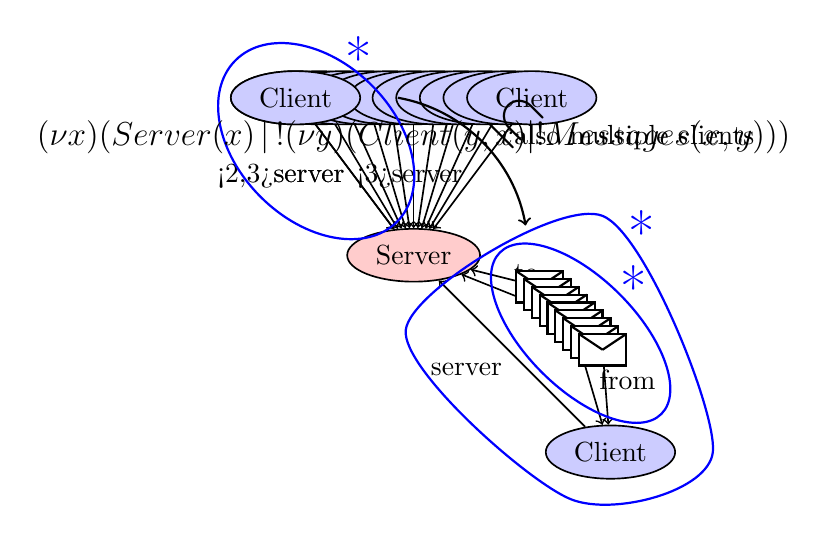
\begin{tikzpicture}[semithick, ->, node distance=2cm]
  \node [draw,ellipse,fill=red!20]  (x) at ( 0, 0) {Server};

  %replication of clients
  \visible<2-4> {
  \node [draw,ellipse,fill=blue!20] (ni) at (-1.5, 2) {Client};
  \path  (ni) edge node [left] {\alt<2,3>{server}{}} (x);
  }

  \visible<4> {
  \node [draw,ellipse,fill=blue!20] (n1) at (-1.2, 2) {Client};
  \path  (n1) edge (x);
  \node [draw,ellipse,fill=blue!20] (n2) at (-0.9, 2) {Client};
  \path  (n2) edge (x);
  \node [draw,ellipse,fill=blue!20] (n3) at (-0.6, 2) {Client};
  \path  (n3) edge (x);
  \node [draw,ellipse,fill=blue!20] (n4) at (-0.3, 2) {Client};
  \path  (n4) edge (x);
  \node [draw,ellipse,fill=blue!20] (n5) at ( 0  , 2) {Client};
  \path  (n5) edge (x);
  \node [draw,ellipse,fill=blue!20] (n6) at ( 0.3, 2) {Client};
  \path  (n6) edge (x);
  \node [draw,ellipse,fill=blue!20] (n7) at ( 0.6, 2) {Client};
  \path  (n7) edge (x);
  \node [draw,ellipse,fill=blue!20] (n8) at ( 0.9, 2) {Client};
  \path  (n8) edge (x);
  \node [draw,ellipse,fill=blue!20] (n9) at ( 1.2, 2) {Client};
  \path  (n9) edge (x);
  }

  \visible<3-4> {
  \node [draw,ellipse,fill=blue!20] (nj) at ( 1.5, 2) {Client};
  \path  (nj) edge node [left] {\alt<3>{server}{}} (x);
  }
  
  \visible<5-12> {
  \node [draw,ellipse,fill=blue!20] (n) at ( -1.5, 2) {Client};
  \path  (n) edge node [left] {server} (x);
  \draw[thick,rotate=45,color=blue] (0.15,1.9) ellipse (1 and 1.45);
  \node[text=blue] (star) at ( -0.7, 2.5) {{\huge *}};
  }
  
  %replication of messages
  \visible<6-> {
  \node [draw,ellipse,fill=blue!20] (m) at ( 2.5, -2.5) {Client};
  \path  (m) edge node [below left] {server} (x);
  }
  
  \visible<7,9-> {
  \tikzMessageNode{mm}{2.0,-0.8}
  \path  (mm) edge node [right] {from} (m);
  \path  (mm) edge node [above right] {to} (x);
  }

  \visible<8> {
  \tikzMessageNode{m1}{1.6,-0.4}
  \tikzMessageNode{m3}{1.7,-0.5}
  \tikzMessageNode{m4}{1.8,-0.6}
  \tikzMessageNode{m5}{1.9,-0.7}
  \tikzMessageNode{m6}{2.0,-0.8}
  \tikzMessageNode{m7}{2.1,-0.9}
  \tikzMessageNode{m8}{2.2,-1.0}
  \tikzMessageNode{m9}{2.3,-1.1}
  \tikzMessageNode{m2}{2.4,-1.2}
  \path  (m2) edge (m);
  \path  (m1) edge (x);
  }

  \visible<9-> {
  \draw[thick,rotate=45,color=blue] (0.8,-2.2) ellipse (0.7 and 1.45);
  \node[text=blue] (star) at ( 2.8, -0.4) {{\huge *}};
  }

  \visible<10-12> {
  \draw[thick] (-.2,2) arc (80:10:2);
  }
  \visible<10> {
  \node (txt1) at ( 2.8, 1.5) {also multiple clients};
  }
  \visible<12> {
  \node[rotate=-45] (txt2) at ( 1.3, 1.7) {{\huge $\subseteq$}};
  }
  
  \visible<11-> {
  \draw[color=blue,thick] plot[smooth cycle] coordinates{(-0.1,-0.95) (2.4,0.5) (3.8,-2.5) (2,-3.1)};
  \node[text=blue] (star) at ( 2.9, 0.3) {{\huge *}};
  }

  \visible<14> {
  \node at (0,1.5) {{\large $(\nu x)(Server(x) \,|\, !(\nu y)(Client(y,x) | !Messages(x,y)))$}};
  }

  \end{tikzpicture}
  \end{figure}
\end{frame}

\begin{frame}
  \frametitle{Motivation: Client-Server system (dynamic topology)}
  \begin{figure}
  \centering
  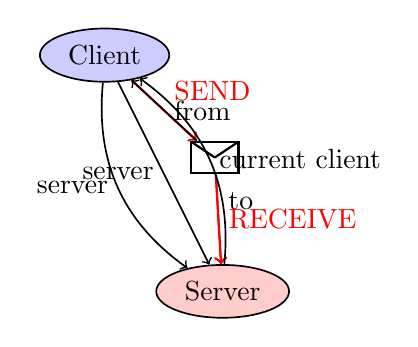
\begin{tikzpicture}[semithick, ->, node distance=2cm]

  \node [draw,ellipse,fill=red!20]  (x) at ( 0, 0) {Server};
  \node [draw,ellipse,fill=blue!20] (ni) at (-1.5, 3) {Client};
  \visible<1-4> {
  \path  (ni) edge node [left] {server} (x);
  }
  
  \visible<2-4> {
  \tikzMessageNode{mm}{-.1,1.7}
  }
  
  \visible<2> {
  \path[thick,color=red]  (ni) edge node [above right] {SEND} (mm);
  }

  \visible<3> {
  \path  (mm) edge node [right] {from} (ni);
  \path  (mm) edge node [above right] {to} (x);
  }
  
  \visible<4> {
  \path[thick,color=red] (mm) edge node [right] {RECEIVE} (x);
  }

  \visible<5> {
  \path  (ni) edge[bend right] node [left] {server} (x);
  \path  (x) edge[bend right] node [right] {current client} (ni);
  }

  \end{tikzpicture}
  \end{figure}
\end{frame}

\begin{frame}
  \frametitle{Covering problem}
  %copy thomas illustration.
  \begin{figure}
  \centering
  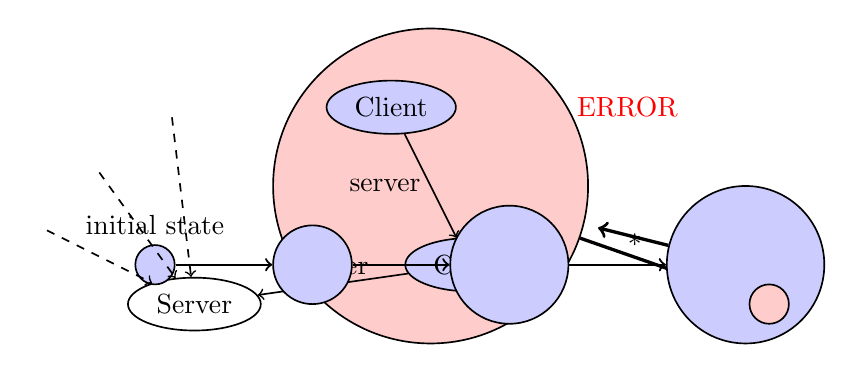
\begin{tikzpicture}[semithick, ->, node distance=2cm]

  \visible<1-2,8> {
  \node[draw,circle,fill=red!20, minimum height=4cm] (err1) at (-0.5,1) {} ;
  \node[color=red] (errlabel) at ( 2, 2) {ERROR};
  \node [draw,ellipse,fill=blue!20]  (x) at ( 0, 0) {Client};
  \node [draw,ellipse,fill=blue!20] (ni) at (-1, 2) {Client};
  \path  (ni) edge node [left] {server} (x);
  \visible<8> {
  \node [draw,ellipse]  (server) at ( -3.5, -0.5) {Server};
  \path  (x) edge node [above] {server} (server);
  }
  }

  \visible<2-5> {
  \node[draw,circle,fill=red!20,minimum height=0.5cm]  (err2) at ( 3.8, -0.5) {};
  }
  \visible<2> {
  \path[very thick] (err1) edge (err2);
  }
  \visible<3-6> {
  \node[draw,circle,fill=blue!20,minimum height=0.5cm]  (init) at ( -4, 0) {};
  }
  \visible<3> {
  \node (initlabel) at ( -4, 0.5) {initial state};
  }
  \visible<4-6> {
  \node[draw,circle,fill=blue!20,minimum height=1cm]  (s1) at ( -2, 0) {};
  \path[thick] (init) edge (s1);
  }
  \visible<5-6> {
  \node[draw,circle,fill=blue!20,minimum height=1.5cm]  (s2) at ( 0.5, 0) {};
  \path[thick] (s1) edge (s2);
  }
  \visible<6-8> {
  \node[draw,circle,fill=blue!20,minimum height=2cm]  (s3) at ( 3.5, 0) {};
  \visible<6>{\path[thick] (s2) edge node [above right] {*} (s3);}
  \node[draw,circle,fill=red!20,minimum height=0.5cm]  (err2) at ( 3.8, -0.5) {};
  }
  \visible<8> {
  \node (invisible) at (1.5,0.5) {};
  \path[very thick] (s3) edge (invisible);
  \begin{scope}
  \node (cli1) at (-3.8,2) {};
  \node (cli2) at (-4.8,1.3) {};
  \node (cli3) at (-5.5,0.5) {};
  \path [dashed] (cli1) edge (server);
  \path [dashed] (cli2) edge (server);
  \path [dashed] (cli3) edge (server);
  \end{scope}
  }

  \end{tikzpicture}
  \end{figure}
\end{frame}

\begin{frame}
  \frametitle{Outline}
  \begin{itemize}
  \item \pical{}, depth-bounded systems
  \item WSTS
  \item Forward/Backward analysis
  \item ADL for depth-bounded systems
  \end{itemize}
%\tableofcontents
\end{frame}

\begin{frame}
  \frametitle{\pical}
  The $\pi$-calculus \cite{DBLP:journals/iandc/MilnerPW92a,DBLP:journals/iandc/MilnerPW92b}
  is a process calculus that describes dynamic distributed computations in a message passing-setting.

\vspace{10pt}

  \[(\nu x)(Server(x) \,|\, (\nu y)(Client(y,x) | Messages(x,y))) \]
  
  \begin{center}
  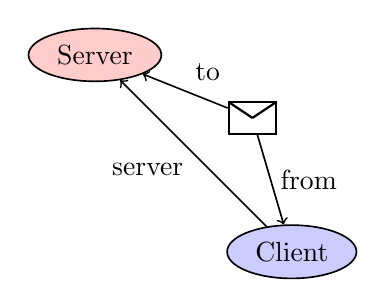
\begin{tikzpicture}[semithick,->]
  \node [draw,ellipse,fill=red!20]  (x) at ( 0, 0) {Server};
  \node [draw,ellipse,fill=blue!20] (m) at ( 2.5, -2.5) {Client};
  \path  (m) edge node [below left] {server} (x);
  \tikzMessageNode{mm}{2.0,-0.8}
  \path  (mm) edge node [right] {from} (m);
  \path  (mm) edge node [above right] {to} (x);
  \end{tikzpicture}
  \end{center}
  
\end{frame}

\iffalse
\begin{frame}
  \frametitle{Communication Topology}
  The configuration of a system of \pical{} equation can be represented as a labelled (bipartite) graph.
  \begin{itemize}
  \item One node per process identifier, labelled by the pid;
  \item One node per name, labelled by $\bullet$;
  \item Labelled edges going from \emph{pid} nodes to \emph{name} nodes.
  The label identifies which parameter the name represents.
  \end{itemize}
\end{frame}

\begin{frame}
  \frametitle{Communication Topology: example}
  $P(x,y) = \overline x(y).P'(x) + \ldots$\\
  $Q(x,z) = x(w).Q'(x,z,w) + \ldots$
  \[
  \genfrac{}{}{}{}{P(x,y) \,|\, Q(x,z)}{\alt<3>{P'(x) \,|\, Q'(x,z,y)}{ }}
  ~~ \genfrac{}{}{0pt}{}{\alt<2->{\rightarrow}{}}{\alt<3->{\leftarrow}{}} ~~
  \visible<2->{
  \genfrac{}{}{}{}{\alert<2>{\overline x(y)}.P'(x) \,|\, \alert<2>{x(w)}.Q'(x,z,w)}{{P'(x) \,|\, Q'(x,z,w)[y/w]}}
  }
  \]

  \vspace{10pt}
  
  $P(1,2) = \overline 1(2).P'(1) + \ldots$\\
  $Q(1,2) = 1(3).Q'(1,2,3) + \ldots$

  %image to represent reduction rule
  \begin{center}
  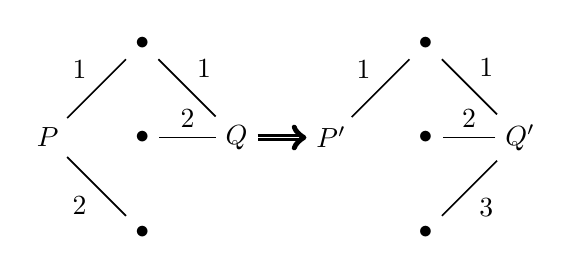
\begin{tikzpicture}[semithick, node distance=1.2cm]
    \node (z) {$\bullet$};
    \node (x) [above of=z] {$\bullet$};
    \node (y) [below of=z] {$\bullet$};
    \node (p) [left of=z] {$P$};
    \node (q) [right of=z] {$Q$};
    \alert<2>{\path (p) edge node [above left] {1} (x);}
    \alert<2>{\path (q) edge node [above right] {1} (x);}
    \path (p) edge node [below left] {2} (y);
    \path (q) edge node [above] {2} (z);

    \visible<3>{
    \node (pp) [right of=q] {$P'$};
    \node (zp) [right of=pp] {$\bullet$};
    \node (xp) [above of=zp] {$\bullet$};
    \node (yp) [below of=zp] {$\bullet$};
    \node (qp) [right of=zp] {$Q'$};
    \path (pp) edge node [above left] {1} (xp);
    \path (qp) edge node [above right] {1} (xp);
    \path (qp) edge node [above] {2} (zp);
    \path (qp) edge node [below right] {3} (yp);

    \path[thick,->] (q) edge[double] (pp);
    }

  \end{tikzpicture}
  \end{center}
\end{frame}
\fi

\begin{frame}
  \frametitle{Client-Server: communication topology}
  \[(\nu x)(Server(x) \,|\, (\nu y)(Client(y,x) | Messages(x,y))) \]
  \begin{eqnarray*}
  Server(self)  & = & self(sender).\ldots \\
  Client(self,server) & = & self().\ldots \\
  Messages(to,from) & = & \overline{to}(from)
  \end{eqnarray*}
  
  \begin{center}
  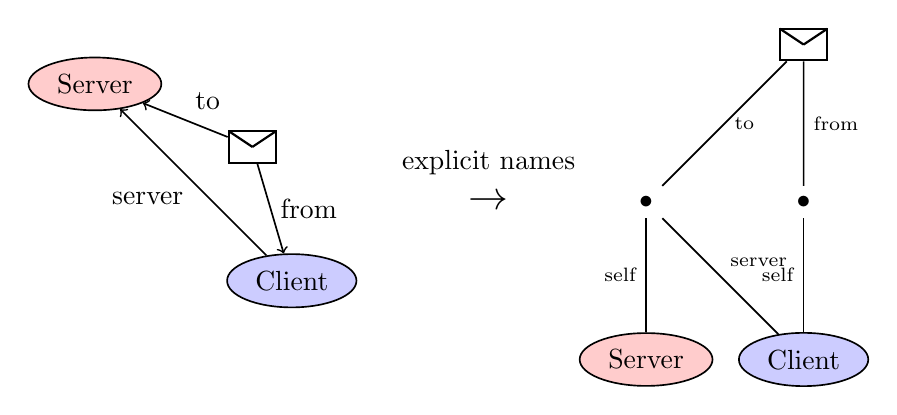
\begin{tikzpicture}[semithick]

  \begin{scope}[xshift=-4cm,->]
  \node [draw,ellipse,fill=red!20]  (x) at ( 0, 0) {Server};

  \node [draw,ellipse,fill=blue!20] (m) at ( 2.5, -2.5) {Client};
  \path  (m) edge node [below left] {server} (x);
  
  \tikzMessageNode{mm}{2.0,-0.8}
  \path  (mm) edge node [right] {from} (m);
  \path  (mm) edge node [above right] {to} (x);
  \end{scope}
  
  \begin{scope}[xshift=1cm,yshift=-1.5cm]
  \node at ( 0, 0.5) {explicit names};
  \node at ( 0, 0) {\Large $\rightarrow$};
  \end{scope}

  \begin{scope}[xshift=3cm, yshift=-3.5cm, node distance=2cm]

  \node [draw,ellipse,fill=red!20]  (x) at ( 0, 0) {Server};
  \node (nx) [above of=x] {$\bullet$};
  \path  (x) edge node [left] {\scriptsize self} (nx);

  \node [draw,ellipse,fill=blue!20] (m) [right of=x] {Client};
  \node (nm) [above of=m] {$\bullet$};
  \path  (m) edge node [left] {\scriptsize self} (nm);
  \path  (m) edge node [above right] {\scriptsize server} (nx);
  
  \tikzMessageNode{mm}{2.0,4}
  \path  (mm) edge node [right] {\scriptsize from} (nm);
  \path  (mm) edge node [right] {\scriptsize to} (nx);
  \end{scope}

  \end{tikzpicture}
  \end{center}
  
\end{frame}

\begin{frame}
  \frametitle{Depth-bounded systems: \cite{Meyer08OnBoundednessInDepth} (1)}
  System with a bound on the longest acyclic path.\\
  (Concretely: it is not possible to encode an infinite memory.)

  \vspace{10pt}

  \begin{figure}
  \centering
  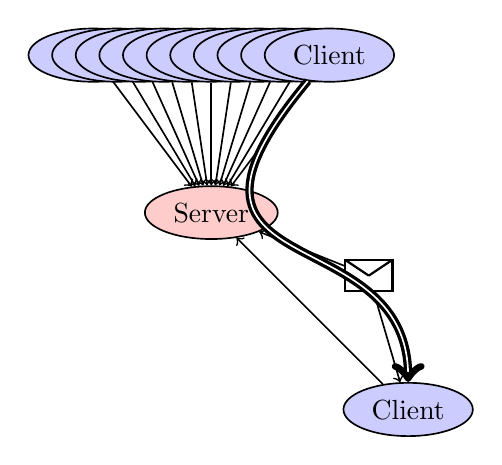
\begin{tikzpicture}[semithick, ->, node distance=2cm]
  \node [draw,ellipse,fill=red!20]  (x) at ( 0, 0) {Server};

  \node [draw,ellipse,fill=blue!20] (ni) at (-1.5, 2) {Client};
  \path  (ni) edge node [left] {} (x);
  \node [draw,ellipse,fill=blue!20] (n1) at (-1.2, 2) {Client};
  \path  (n1) edge (x);
  \node [draw,ellipse,fill=blue!20] (n2) at (-0.9, 2) {Client};
  \path  (n2) edge (x);
  \node [draw,ellipse,fill=blue!20] (n3) at (-0.6, 2) {Client};
  \path  (n3) edge (x);
  \node [draw,ellipse,fill=blue!20] (n4) at (-0.3, 2) {Client};
  \path  (n4) edge (x);
  \node [draw,ellipse,fill=blue!20] (n5) at ( 0  , 2) {Client};
  \path  (n5) edge (x);
  \node [draw,ellipse,fill=blue!20] (n6) at ( 0.3, 2) {Client};
  \path  (n6) edge (x);
  \node [draw,ellipse,fill=blue!20] (n7) at ( 0.6, 2) {Client};
  \path  (n7) edge (x);
  \node [draw,ellipse,fill=blue!20] (n8) at ( 0.9, 2) {Client};
  \path  (n8) edge (x);
  \node [draw,ellipse,fill=blue!20] (n9) at ( 1.2, 2) {Client};
  \path  (n9) edge (x);
  \node [draw,ellipse,fill=blue!20] (nj) at ( 1.5, 2) {Client};
  \path  (nj) edge node [left] {} (x);
  
  \node [draw,ellipse,fill=blue!20] (m) at ( 2.5, -2.5) {Client};
  \path  (m) edge node [below left] {} (x);
  
  \tikzMessageNode{mm}{2.0,-0.8}
  \path  (mm) edge node [right] {} (m);
  \path  (mm) edge node [above right] {} (x);

  \draw[very thick,double] (nj) .. controls (-1,-1) and (2.5,0) .. (m);

  \end{tikzpicture}
  \end{figure}
\end{frame}

\begin{frame}
  \frametitle{Depth-bounded systems: \cite{Meyer08OnBoundednessInDepth} (2)}

  \begin{figure}
  \centering
  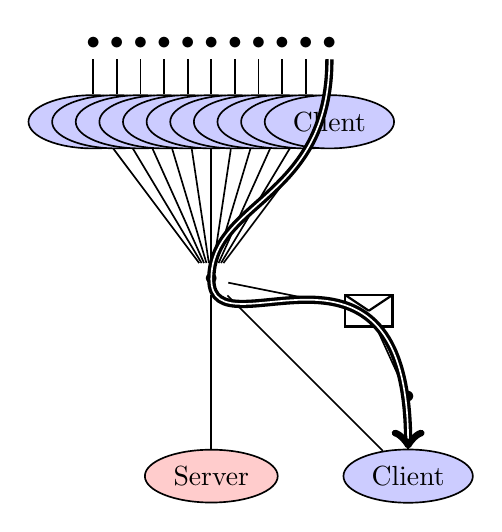
\begin{tikzpicture}[semithick, node distance=2cm]
  \node (x) at ( 0, 0) {$\bullet$};
  \node [draw,ellipse,fill=red!20]  (server) at ( 0, -2.5) {Server};
  \path  (server) edge (x);

  %replication of clients
  \node [draw,ellipse,fill=blue!20] (ni) at (-1.5, 2) {Client};
  \path  (ni) edge (x);
  \node  (nni) at (-1.5, 3) {$\bullet$};
  \path  (ni) edge (nni);
  \node [draw,ellipse,fill=blue!20] (n1) at (-1.2, 2) {Client};
  \path  (n1) edge (x);
  \node  (nn1) at (-1.2, 3) {$\bullet$};
  \path  (n1) edge (nn1);
  \node [draw,ellipse,fill=blue!20] (n2) at (-0.9, 2) {Client};
  \path  (n2) edge (x);
  \node  (nn2) at (-0.9, 3) {$\bullet$};
  \path  (n2) edge (nn2);
  \node [draw,ellipse,fill=blue!20] (n3) at (-0.6, 2) {Client};
  \path  (n3) edge (x);
  \node  (nn3) at (-0.6, 3) {$\bullet$};
  \path  (n3) edge (nn3);
  \node [draw,ellipse,fill=blue!20] (n4) at (-0.3, 2) {Client};
  \path  (n4) edge (x);
  \node  (nn4) at (-0.3, 3) {$\bullet$};
  \path  (n4) edge (nn4);
  \node [draw,ellipse,fill=blue!20] (n5) at ( 0  , 2) {Client};
  \path  (n5) edge (x);
  \node  (nn5) at (-0.0, 3) {$\bullet$};
  \path  (n5) edge (nn5);
  \node [draw,ellipse,fill=blue!20] (n6) at ( 0.3, 2) {Client};
  \path  (n6) edge (x);
  \node  (nn6) at (0.3, 3) {$\bullet$};
  \path  (n6) edge (nn6);
  \node [draw,ellipse,fill=blue!20] (n7) at ( 0.6, 2) {Client};
  \path  (n7) edge (x);
  \node  (nn7) at (0.6, 3) {$\bullet$};
  \path  (n7) edge (nn7);
  \node [draw,ellipse,fill=blue!20] (n8) at ( 0.9, 2) {Client};
  \path  (n8) edge (x);
  \node  (nn8) at (0.9, 3) {$\bullet$};
  \path  (n8) edge (nn8);
  \node [draw,ellipse,fill=blue!20] (n9) at ( 1.2, 2) {Client};
  \path  (n9) edge (x);
  \node  (nn9) at (1.2, 3) {$\bullet$};
  \path  (n9) edge (nn9);
  \node [draw,ellipse,fill=blue!20] (nj) at ( 1.5, 2) {Client};
  \path  (nj) edge (x);
  \node  (nnj) at (1.5, 3) {$\bullet$};
  \path  (nj) edge (nnj);
  
  \node [draw,ellipse,fill=blue!20] (m) at ( 2.5, -2.5) {Client};
  \path  (m) edge (x);
  \node  (nm) at (2.5, -1.5) {$\bullet$};
  \path  (m) edge (nm);
  
  \tikzMessageNode{mm}{2.0,-0.4}
  \path  (mm) edge node [right] {} (nm);
  \path  (mm) edge node [above right] {} (x);

  \visible<2>{
  \draw[very thick,double,->] (nnj) .. controls  (1.5,1) and (0,1) .. (0,0) .. controls (0,-1) and (2.5,1) .. (m);
  }

  \end{tikzpicture}
  \end{figure}
\end{frame}

\begin{frame}
  \frametitle{About Depth-bounded systems}
  \begin{itemize}
  \item Depth-bounded systems are well-structured transition systems \cite{Meyer08OnBoundednessInDepth}.
  \item Reachability is undecidable.
  \item Termination is decidable.
  \item Coverability is decidable for system of known depth.
  \item Coverability for any depth-bounded system was an open problem.
  \end{itemize}

  \vspace{10pt}

  Our contribution:\\
  Coverability is decidable for any depth-bounded system.

\end{frame}

\begin{frame}
  \frametitle{Well-structured transition system}
  A well-structured transition system (WSTS)
  is a transition system $\langle S, \rightarrow, \leq \rangle$ such that:
  \begin{itemize}
  \item
    $\leq$ is a well-quasi-ordering (wqo),\\
    i.e. well-founded + no infinite antichain.
  \item
    compatibility of $\leq$ w.r.t. $\rightarrow$\\
    \begin{center}
    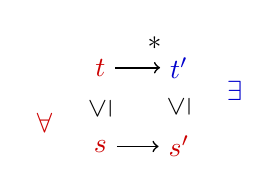
\begin{tikzpicture}[semithick, ->]
    \node[color=red!80!black] (s) {$s$};
    \node[color=red!80!black] (t) [above of=s] {$t$};
    \node[color=red!80!black] (sp) [right of=s] {$s'$};
    \node[color=blue!80!black] (tp) [right of=t] {$t'$};

    \path[color=white]  (s) edge node[color=black,rotate=90] {$\leq$} (t);
    \path  (s) edge (sp);
    \path  (t) edge node [above right] {*} (tp);
    \path[color=white]  (sp) edge node[color=black,rotate=90] {$\leq$} (tp);
    
    \node[color=blue!80!black] (exists) [above right of=sp] {$\exists$};
    \node[color=red!80!black] (forall) [below left of=t] {$\forall$};

    \end{tikzpicture}
    \end{center}
  \end{itemize}

  for more detail see: \cite{DBLP:journals/tcs/FinkelS01, DBLP:conf/lics/AbdullaCJT96}

  \vspace{5pt}

  A better-quasi-ordering is a wqo closed under the powerset construction.

  \vspace{5pt}
  
  $\uparrow x = \{ x' \in S \,|\, x \leq x' \}$ is an upward-closed set.\\
  $\downarrow x = \{ x' \in S \,|\, x' \leq x \}$ is an downward-closed set.
\end{frame}

\begin{frame}
  \frametitle{Depth bounded systems as WSTS}
  \cite{Meyer08OnBoundednessInDepth} showed that depth-bounded processes are WSTS for
  \begin{itemize}
  \item their \emph{reachable} configurations and
  \item the quasi-ordering $\subgraph$ induced by \emph{subgraph isomorphism}.
  \end{itemize}

  \begin{center}
  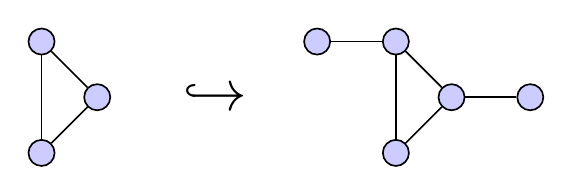
\begin{tikzpicture}[semithick]

  \begin{scope}[xshift=-1.5cm]
    \node[circle,draw,fill=blue!20] (n1) at (0,0) { };
    \node[circle,draw,fill=blue!20] (n2) [above left of=n1] { };
    \node[circle,draw,fill=blue!20] (n3) [below left of=n1] { };
    \path (n1) edge (n2);
    \path (n1) edge (n3);
    \path (n2) edge (n3);
  \end{scope}

  \node at (0,0) {\huge $\subgraph$};
  
  \begin{scope}[xshift=3cm]
    \node[circle,draw,fill=blue!20] (n1) at (0,0) { };
    \node[circle,draw,fill=blue!20] (n2) [above left of=n1] { };
    \node[circle,draw,fill=blue!20] (n3) [below left of=n1] { };
    \node[circle,draw,fill=blue!20] (n4) [right of=n1] { };
    \node[circle,draw,fill=blue!20] (n5) [left of=n2] { };
    \path (n1) edge (n2);
    \path (n1) edge (n3);
    \path (n2) edge (n3);
    \path (n1) edge (n4);
    \path (n2) edge (n5);
  \end{scope}

  \end{tikzpicture}
  \end{center}

  \cite{Meyer08OnBoundednessInDepth} showed that $\subgraph$ is a well-quasi-ordering on the reachable configurations.\\
  We show that it is a better-quasi-ordering.

\end{frame}

%TODO tree closure
\begin{frame}
  \frametitle{Tree-Depth of a graph}

  \begin{block}{Tree-Depth}
  The tree-depth td(G) of a graph G is the minimal height of all trees whose closure contains G.
  \end{block}

  \begin{center}
  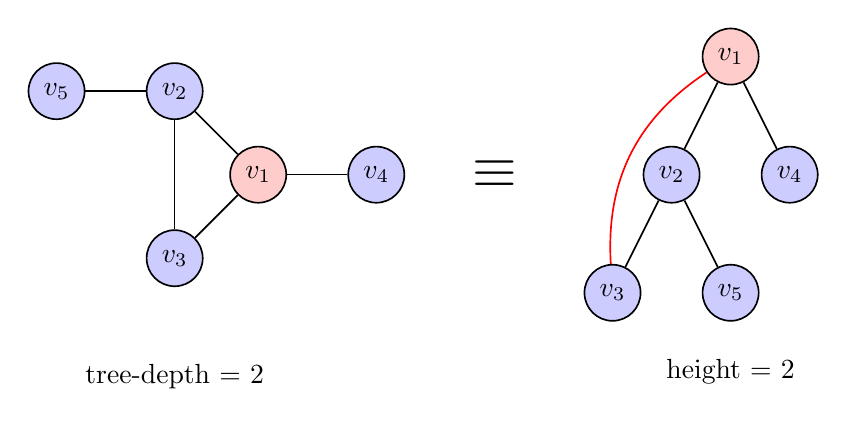
\begin{tikzpicture}[semithick]

  \begin{scope}[xshift=-3cm,node distance=1.5cm]
    \node[circle,draw,fill=red!20] (n1) at (0,0) {$v_1$};
    \node[circle,draw,fill=blue!20] (n2) [above left of=n1] {$v_2$};
    \node[circle,draw,fill=blue!20] (n3) [below left of=n1] {$v_3$};
    \node[circle,draw,fill=blue!20] (n4) [right of=n1] {$v_4$};
    \node[circle,draw,fill=blue!20] (n5) [left of=n2] {$v_5$};
    \path (n1) edge (n2);
    \path (n1) edge (n3);
    \path (n2) edge (n3);
    \path (n1) edge (n4);
    \path (n2) edge (n5);

    \node [below of=n3] {tree-depth = 2};
  \end{scope}

  \node at (0,0) {\huge $\equiv$};
  
  \begin{scope}[xshift=3cm, yshift=1.5cm]
    \node[circle,draw,fill=red!20] (n1) {$v_1$}
      child{ node[circle,draw,fill=blue!20] (n2) {$v_2$}
        child{node[circle,draw,fill=blue!20] (n3) {$v_3$}}
        child{node[circle,draw,fill=blue!20] (n5) {$v_5$}}
      }
      child{node[circle,draw,fill=blue!20] (n4) {$v_4$}};
    \path[red] (n1) edge[bend right] (n3);
    
    \node [below of=n5] {height = 2};
  \end{scope}

  \end{tikzpicture}
  \end{center}
\end{frame}

\begin{frame}
  \frametitle{Tree encoding of depth bounded graph}

  \begin{center}
  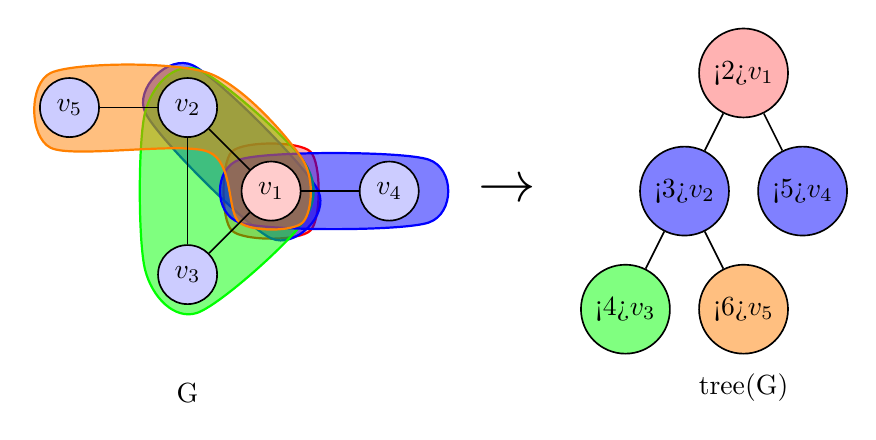
\begin{tikzpicture}[semithick]

  \begin{scope}[xshift=-3cm,node distance=1.5cm]
    \visible<2>{
      \draw[color=red,fill=red,thick,fill opacity=0.3] plot[smooth cycle]
      coordinates{(-0.5,-0.5) (-0.5,0.5) (0.5,0.5) (0.5,-0.5)};
    }
    \visible<3>{
      \draw[color=blue,fill=blue,thick,fill opacity=0.5] plot[smooth cycle]
      coordinates{(-1.6,1) (-1,1.6) (0.6,0) (0,-0.6)};
    }
    \visible<4>{
      \draw[color=green,fill=green,thick,fill opacity=0.5] plot[smooth cycle]
      coordinates{(-1.6,1) (-0.95,1.55) (0.4,0.4) (0.4,-0.4) (-0.95,-1.55) (-1.6,-1)};
    }
    \visible<5>{
      \draw[color=blue,fill=blue,thick,fill opacity=0.5] plot[smooth cycle]
      coordinates{(-0.4,-0.4) (-0.4,0.4) (2,0.4) (2,-0.4)};
    }
    \visible<6>{
      \draw[color=orange,fill=orange,thick,fill opacity=0.5] plot[smooth cycle]
      coordinates{(-2.8, 0.55) (-2.8, 1.5) (-0.8,1.5) (0.4,0.4) (0.4,-0.4) (-0.4, -0.4) (-0.8, 0.5)};
    }
    \node[minimum height=0.75cm,circle,draw,fill=red!20] (n1) at (0,0) {$v_1$};
    \node[minimum height=0.75cm,circle,draw,fill=blue!20] (n2) [above left of=n1] {$v_2$};
    \node[minimum height=0.75cm,circle,draw,fill=blue!20] (n3) [below left of=n1] {$v_3$};
    \node[minimum height=0.75cm,circle,draw,fill=blue!20] (n4) [right of=n1] {$v_4$};
    \node[minimum height=0.75cm,circle,draw,fill=blue!20] (n5) [left of=n2] {$v_5$};
    \path (n1) edge (n2);
    \path (n1) edge (n3);
    \path (n2) edge (n3);
    \path (n1) edge (n4);
    \path (n2) edge (n5);
    \node [below of=n3] {G};
  \end{scope}

  \node at (0,0) {\huge $\rightarrow$};
  
  \begin{scope}[xshift=3cm, yshift=1.5cm]
    \node[circle,draw,fill=red!30] (n1) {\alert<2>{$v_1$}}
      child{ node[circle,draw,fill=blue!50] (n2) {\alert<3>{$v_2$}}
        child{node[circle,draw,fill=green!50] (n3) {\alert<4>{$v_3$}}}
        child{node[circle,draw,fill=orange!50] (n5) {\alert<6>{$v_5$}}}
      }
      child{node[circle,draw,fill=blue!50] (n4) {\alert<5>{$v_4$}}};
    \node [below of=n5] {tree(G)};
  \end{scope}

  \end{tikzpicture}
  \end{center}

  \vspace{10pt}

  The labels of tree(G) are graphs.\\
  The \alert{number of labels} used in the encodings is \alert{finite}.
\end{frame}

\begin{frame}
  \frametitle{Homeomorphic tree embedding}
  \begin{center}
  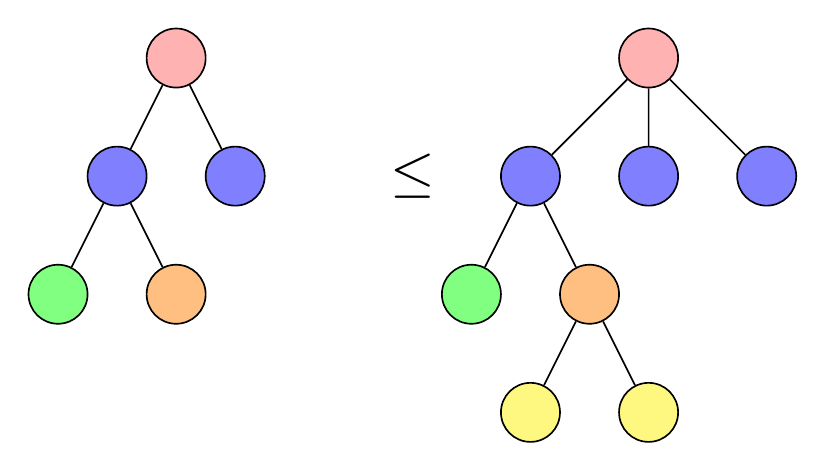
\begin{tikzpicture}[semithick]

  \begin{scope}[xshift=-3cm, yshift=1.5cm]
    \node[minimum height=0.75cm,circle,draw,fill=red!30] (n1) {}
      child{ node[minimum height=0.75cm,circle,draw,fill=blue!50] (n2) {}
        child{node[minimum height=0.75cm,circle,draw,fill=green!50] (n3) {}}
        child{node[minimum height=0.75cm,circle,draw,fill=orange!50] (n5) {}}
      }
      child{node[minimum height=0.75cm,circle,draw,fill=blue!50] (n4) {}};
  \end{scope}

  \node at (0,0) {\huge $\leq$};
  
  \begin{scope}[xshift=3cm, yshift=1.5cm]
    \node[minimum height=0.75cm,circle,draw,fill=red!30] (n1) {}
      child{node[minimum height=0.75cm,circle,draw,fill=blue!50] (n2) {}
        child{node[minimum height=0.75cm,circle,draw,fill=green!50] (n3) {}}
        child{node[minimum height=0.75cm,circle,draw,fill=orange!50] (n5) {}
          child{node[minimum height=0.75cm,circle,draw,fill=yellow!50] (n7) {}}
          child{node[minimum height=0.75cm,circle,draw,fill=yellow!50] (n8) {}}
        }
      }
      child{node[minimum height=0.75cm,circle,draw,fill=blue!50] (n4) {}}
      child{node[minimum height=0.75cm,circle,draw,fill=blue!50] (n6) {}};
  \end{scope}

  \end{tikzpicture}
  \end{center}

  \vspace{10pt}

  We can show for all graphs G$_1$, G$_2$:\\
  \begin{center}
    tree(G$_1$) $\leq$ tree(G$_2$) implies G$_1$ $\subgraph$ G$_2$
  \end{center}
\end{frame}

\begin{frame}
  \frametitle{Kruskal's tree theorem}
  \begin{block}{Extension of Kruskal's tree theorem \cite{Laver71OnFraissesOrderTypeConjecture}}
  Homeomorphic tree embedding is a better-quasi-ordering on finite trees, where the labels are better-quasi-ordered.
  \end{block}

  \vspace{10pt}

  \begin{block}{Proposition}
  Labelled graphs of bounded tree-depth are better-quasi-orderered by the relation induced by subgraph isomorphisms.
  \end{block}

  \vspace{10pt}

  $\Rightarrow$ Subgraph isomorphisms induce a better-quasi-ordering on the reachable configurations of a depth-bounded system.
\end{frame}

\begin{frame}
  \frametitle{Backward analysis}
  %thomas illustration of pre*
  \begin{center}
  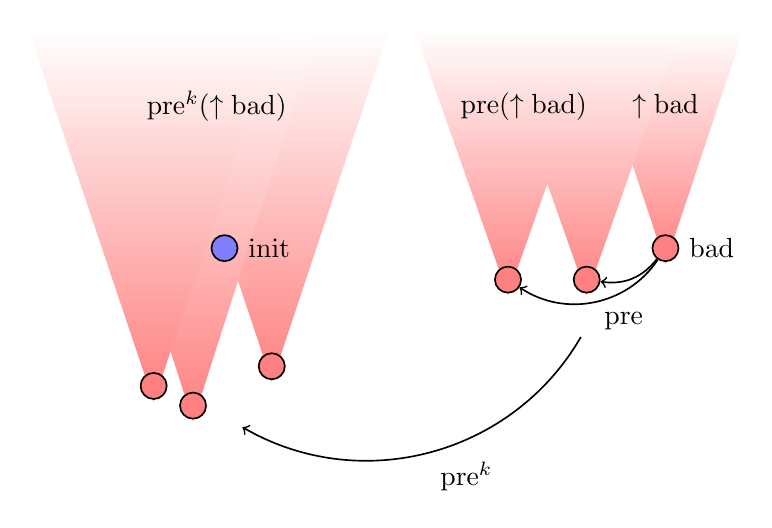
\begin{tikzpicture}[semithick,->]

  \shade[bottom color=red!50,top color=white] (3,5) -- (4,2) -- (5,5);
  \node[draw,circle,fill=red!50,minimum height=0.2,label={right:bad}] (e1) at (4,2.2) {};

  \visible<2->{
  \shade[bottom color=red!50,top color=white] (1.8,5) -- (3,1.6) -- (4.2,5);
  \node[draw,circle,fill=red!50,minimum height=0.2] (e2) at (3,1.8) {};
  \shade[bottom color=red!50,top color=white] (0.8,5) -- (2,1.6) -- (3.2,5);
  \node[draw,circle,fill=red!50,minimum height=0.2] (e3) at (2,1.8) {};
  \path (e1) edge[bend left] (e2);
  \path (e1) edge[bend left=45] node[below right] {pre} (e3);
  \node at (2.2,4) {$\text{pre}(\uparrow\text{bad})$};
  }

  \visible<3->{
  \shade[bottom color=red!50,top color=white] (-2.5,5) -- (-1,0.5) -- (0.5,5);
  \node[draw,circle,fill=red!50,minimum height=0.2] at (-1,0.7) {};
  \shade[bottom color=red!50,top color=white] (-3.6,5) -- (-2,0) -- (-0.4,5);
  \node[draw,circle,fill=red!50,minimum height=0.2] at (-2,0.2) {};
  \shade[bottom color=red!50,top color=white] (-4.1,5) -- (-2.5,0.25) -- (-0.9,5);
  \node[draw,circle,fill=red!50,minimum height=0.2] at (-2.5,0.45) {};

  \node (e4) at (3,1.2) {};
  \node (e5) at (-1.5,0) {};
  \path (e4) edge[bend left=45] node[below right] {pre$^k$} (e5);
  \node at (-1.7,4) {$\text{pre}^k(\uparrow\text{bad})$};
  }

  \visible<4->{
  \node[draw,circle,fill=blue!50,minimum height=0.2,label={right:init}] at (-1.6,2.2) {};
  }
  
  %on top of the shades
  \node at (4,4) {$\uparrow\text{bad}$};
  
  \end{tikzpicture}
  \end{center}
\end{frame}

\begin{frame}
  \frametitle{Analysis of depth-bounded systems: Backward analysis}

  \begin{itemize}
  \item Backward analysis requires \emph{pre} to be computable.
  \item The WSTS of a depth-bounded system is defined wrt. the \emph{forward-reachable} configurations.
  \item pre generates unreachable configurations.
  \item The set of reachable configurations is not computable
  \item We need to known the depth to preserve the wqo.
  \item Backward algorithms for coverability works only with processes of \emph{known depth}.
  \end{itemize}

\end{frame}

%picture with reachable states, k-bounded configuration, pre that diverges.
\begin{frame}
  \frametitle{Analysis of depth-bounded systems: computing \emph{pre}}
  
  \begin{center}
  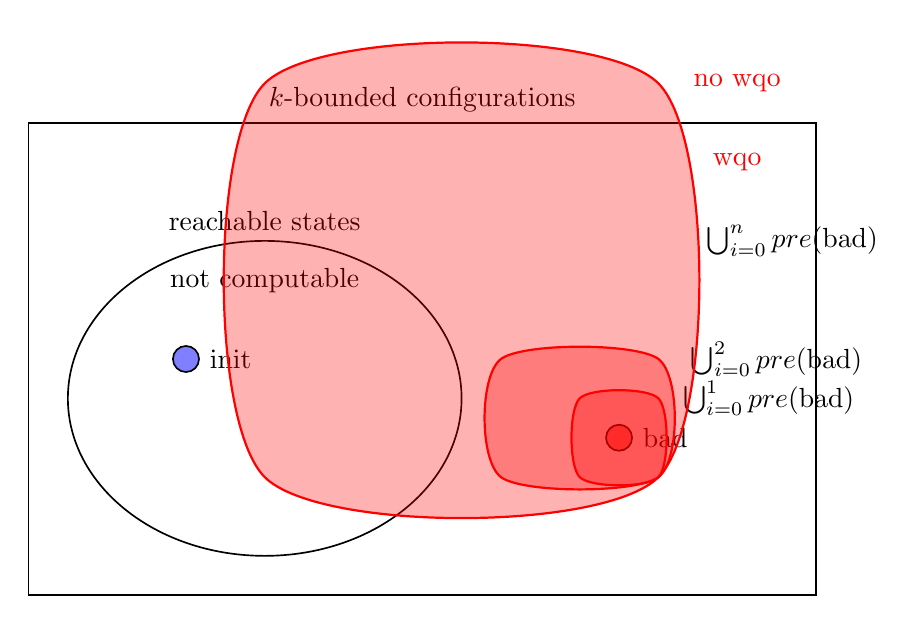
\begin{tikzpicture}[semithick]
  
  \visible<3->{\node [draw,minimum height=6cm,minimum width=10cm,label={above:$k$-bounded configurations}] (x) at ( 0, 0) {};}
  \node [draw,ellipse,minimum height=4cm,minimum width=5cm,label={above:reachable states}] (y) at ( -2, -0.5) {};
  
  \visible<3->{\node [red] (v) at ( 4, 2.5) {wqo};}
  \visible<3->{\node [red] (w) at ( 4, 3.5) {no wqo};}
  \visible<2->{\node (c) at ( -2, 1) {not computable};}
  
  \node[draw,circle,fill=red!50,minimum height=0.2,label={right:bad}] (e1) at (2.5,-1) {};
  \node[draw,circle,fill=blue!50,minimum height=0.2,label={right:init}] (e2) at (-3,0) {};

  \visible<4->{
  \draw[color=red,fill=red,thick,fill opacity=0.3] plot[smooth cycle]
  coordinates{(3,-1.5) (2,-1.5) (2,-0.5) (3,-0.5)};
  \node at ( 4.4, -0.5) {$\bigcup_{i=0}^1 pre(\text{bad})$};
  }
  
  \visible<5->{
  \draw[color=red,fill=red,thick,fill opacity=0.3] plot[smooth cycle]
  coordinates{(3,-1.5) (1,-1.5) (1,0) (3,0)};
  \node at ( 4.5, 0) {$\bigcup_{i=0}^2 pre(\text{bad})$};
  }
  
  \visible<6->{
  \draw[color=red,fill=red,thick,fill opacity=0.3] plot[smooth cycle]
  coordinates{(3,-1.5) (-2,-1.5) (-2,3.5) (3,3.5)};
  \node at ( 4.7, 1.5) {$\bigcup_{i=0}^n pre(\text{bad})$};
  }

  \end{tikzpicture}
  \end{center}

\end{frame}

\begin{frame}
  \frametitle{Forward analysis}
  %thomas illustration of post*
  \begin{center}
  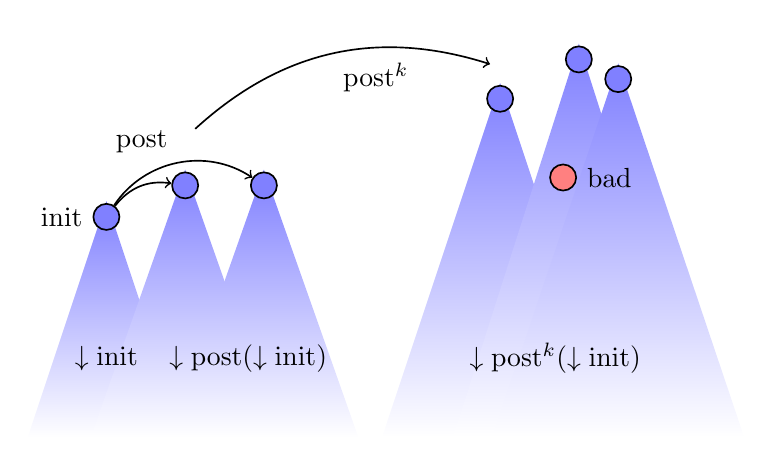
\begin{tikzpicture}[semithick,->]

  \shade[top color=blue!50,bottom color=white] (-3,-5) -- (-4,-2) -- (-5,-5);
  \node[draw,circle,fill=blue!50,minimum height=0.2,label={left:init}] (e1) at (-4,-2.2) {};

  \visible<2->{
  \shade[top color=blue!50,bottom color=white] (-1.8,-5) -- (-3,-1.6) -- (-4.2,-5);
  \node[draw,circle,fill=blue!50,minimum height=0.2] (e2) at (-3,-1.8) {};
  \shade[top color=blue!50,bottom color=white] (-0.8,-5) -- (-2,-1.6) -- (-3.2,-5);
  \node[draw,circle,fill=blue!50,minimum height=0.2] (e3) at (-2,-1.8) {};
  \path (e1) edge[bend left] (e2);
  \path (e1) edge[bend left=45] node[above left] {post} (e3);
  \node at (-2.2,-4) {$\downarrow\text{post}(\downarrow\text{init})$};
  }

  \visible<3->{
  \shade[top color=blue!50,bottom color=white] (2.5,-5) -- (1,-0.5) -- (-0.5,-5);
  \node[draw,circle,fill=blue!50,minimum height=0.2] at (1,-0.7) {};
  \shade[top color=blue!50,bottom color=white] (3.6,-5) -- (2,0) -- (0.4,-5);
  \node[draw,circle,fill=blue!50,minimum height=0.2] at (2,-0.2) {};
  \shade[top color=blue!50,bottom color=white] (4.1,-5) -- (2.5,-0.25) -- (0.9,-5);
  \node[draw,circle,fill=blue!50,minimum height=0.2] at (2.5,-0.45) {};

  \node (e4) at (-3,-1.2) {};
  \node (e5) at (1,-0.3) {};
  \path (e4) edge[bend left] node[below right] {post$^k$} (e5);
  \node at (1.7,-4) {$\downarrow\text{post}^k(\downarrow\text{init})$};
  }

  \visible<4->{
  \node[draw,circle,fill=red!50,minimum height=0.2,label={right:bad}] at (1.8,-1.7) {};
  }
  %on top of the shades
  \node at (-4,-4) {$\downarrow\text{init}$};
  \end{tikzpicture}
  \end{center}
  \begin{block}<5>{Problem}
  How to represents downward-closed sets ?
  \end{block}
\end{frame}

\begin{frame}
  \frametitle{Analysis of depth-bounded systems: Forward analysis}

  \begin{itemize}
  \item Forward algorithms terminate even if the \emph{bound is not known}.
  \item The algorithm is an instance of the expand enlarge check algorithm \cite{GeeraertsETAL06ExpandEnlargeCheck} that uses \alert{adequate domain of limits} (ADL).
  \item \cite{FinkelGoubaultLarrecq09ForwardAnalysisForWSTS} provides a theoretical framework for the manipulation of downward-closed sets and the construction of ADL.
  \item We build such an ADL by extending configurations with `!'.
  \end{itemize}

  \vspace{10pt}

  $\Rightarrow$ coverability is decidable for the entire class of depth-bounded systems.
\end{frame}


\begin{frame}
  \frametitle{Adequate Domain of Limit (1)}
  ADL: \cite{GeeraertsETAL06ExpandEnlargeCheck}\\
  let $Y$ an ADL for wqo set $X$:
  \[\text{For every} ~ z \in \text{X} \cup \text{Y}, \gamma(z) ~ \text{is a downward-closed subset of X}.\]

  \begin{center}
  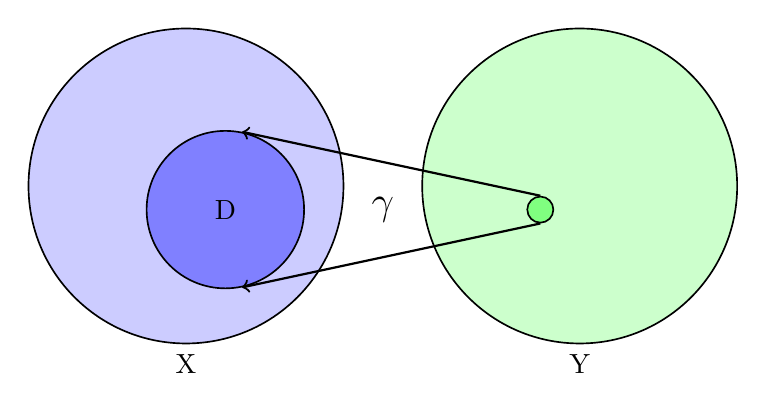
\begin{tikzpicture}[semithick, ->]
  \node [draw,circle,fill=blue!20, minimum height=4cm, label={below:X}] at ( -2.5, 0) {};
  \node [draw,circle,fill=green!20, minimum height=4cm, label={below:Y}] at ( 2.5, 0) {};
  
  \node [draw,circle,fill=green!50] (a) at ( 2, -0.3) {};
  \node [draw,circle,fill=blue!50, minimum height=2cm] (b) at ( -2, -0.3) {D};
  \draw[thick] (a.north) -- (tangent cs:node=b,point={(a.north)},solution=1);
  \draw[thick] (a.south) -- (tangent cs:node=b,point={(a.south)},solution=2);
  \node at ( 0, -0.3) {\Large $\gamma$};

  \end{tikzpicture}
  \end{center}
\end{frame}

\begin{frame}
  \frametitle{Adequate Domain of Limit (2)}
  \begin{center}
    Every downward-closed subset D of X is\\
    generated by a finite subset E of Y $\cup$ X.
  \end{center}

  \begin{center}
  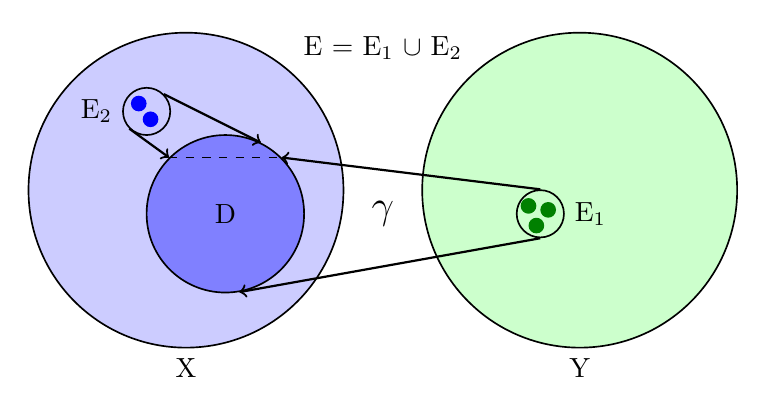
\begin{tikzpicture}[semithick]
  \node [draw,circle,fill=blue!20, minimum height=4cm, label={below:X}] at ( -2.5, 0) {};
  \node [draw,circle,fill=green!20, minimum height=4cm, label={below:Y}] at ( 2.5, 0) {};
  
  \node [draw,circle,minimum height=6mm,label={right:E$_1$}] (a) at ( 2, -0.3) {};
  \node[circle,fill=green!50!black,inner sep=2pt] at (2.1, -0.25) {};
  \node[circle,fill=green!50!black,inner sep=2pt] at (1.95, -0.45) {};
  \node[circle,fill=green!50!black,inner sep=2pt] at (1.85, -0.2) {};
  \node [draw,circle,fill=blue!50, minimum height=2cm] (b) at ( -2, -0.3) {D};
  \draw[dashed] (b.north west) -- (b.north east);
  \draw[thick,->] (a.north) -- (b.north east);
  \draw[thick,->] (a.south) -- (tangent cs:node=b,point={(a.south)},solution=2);
  \node at ( 0, -0.3) {\Large $\gamma$};
  
  \node at ( 0, 1.8) {E = E$_1$ $\cup$ E$_2$};

  \node [draw,circle,minimum height=6mm,label={left:E$_2$}] (c) at ( -3, 1) {};
  \node[circle,fill=blue,inner sep=2pt] at (-3.1, 1.1) {};
  \node[circle,fill=blue,inner sep=2pt] at (-2.95, 0.9) {};
  \draw[thick,->] (c.north east) -- (tangent cs:node=b,point={(c.north east)},solution=2);
  \draw[thick,->] (c.south west) -- (b.north west);


  \end{tikzpicture}
  \end{center}
\end{frame}

\againframe<14>{clientServer1}

\begin{frame}
  \frametitle{Limits configuration for depth-bounded systems}
  We use \alert{`!'} not as a recursion operator but as a mean to represent infinite sets of configurations.

  \vspace{10pt}

  \alert{$\mathcal{C(}PI , k)$} is the set of configurations.\\
  \alert{$\mathcal{L(}PI , k)$} in the set of limit configurations.

  \begin{block}{Theorem}
  Let $k \in \mathbb{N}$ and let $PI$ be a finite set of process identifiers.
  Then $(\mathcal{L(}PI , k), \sqsubseteq, \gamma)$ is a weak adequate domain of limits
  for the well-quasi-ordered set $(\mathcal{C}(PI , k), \leq)$.
  \end{block}

  \begin{block}{Corollary}
  Coverability is decidable for the entire class of depth-bounded systems.
  \end{block}

\end{frame}

%overview of the proof and goubault-larec thm
%For this purpose we show
%that downward-closed sets of configurations in depth-bounded processes are character-
%ized by finite unions of regular languages of unranked trees.
\begin{frame}
  \frametitle{Limits configuration for depth-bounded systems}
  \begin{block}{Theorem \cite{FinkelGoubaultLarrecq09ForwardAnalysisForWSTS}}
  The downward-closed directed subsets of a wqo set X form an ADL for X.
  \end{block}

  %ideals always exists.
  \begin{center}
  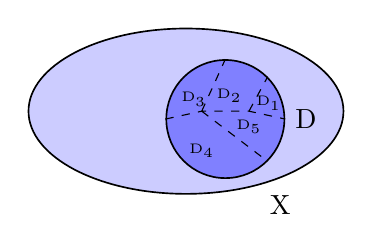
\begin{tikzpicture}[semithick]
  \node [draw,ellipse,fill=blue!20, minimum height=2.1cm, minimum width=4cm, label={below right:X}] {};
  \node [draw,circle,fill=blue!50, minimum height=1.5cm, label={right:D}] (d) at ( 0.5, -0.1) {};
  \coordinate (c1) at (0.2,0);
  \coordinate (c2) at (0.8,0);
  \draw[dashed,thin]
    (d.west) -- (c1) -- (c2) -- (d.east)
    (c1) -- (d.north)
    (c2) -- (d.north east)
    (c1) -- (d.south east)
  ;
  \node at (1.05,0.1) {\tiny D$_1$};
  \node at (0.55,0.2) {\tiny D$_2$};
  \node at (0.1,0.15) {\tiny D$_3$};
  \node at (0.2,-0.5) {\tiny D$_4$};
  \node at (0.8,-0.2) {\tiny D$_5$};
  \end{tikzpicture}
  \end{center}

  \begin{block}{Proposition}
  The directed downward-closed sets of depth-bounded configurations are exactly the denotations of limit configurations.
  \end{block}

  We characterize the tree encodings of downward-closed sets of configurations in terms of the languages of \emph{hedge automata}.
\end{frame}


\begin{frame}
  \frametitle{Regular language of unranked trees for Client-Server (1)}
  \[(\nu x)(Server(x) \,|\, !(\nu y)(Client(y,x) | !Messages(x,y))) \]
  
  \begin{center}
  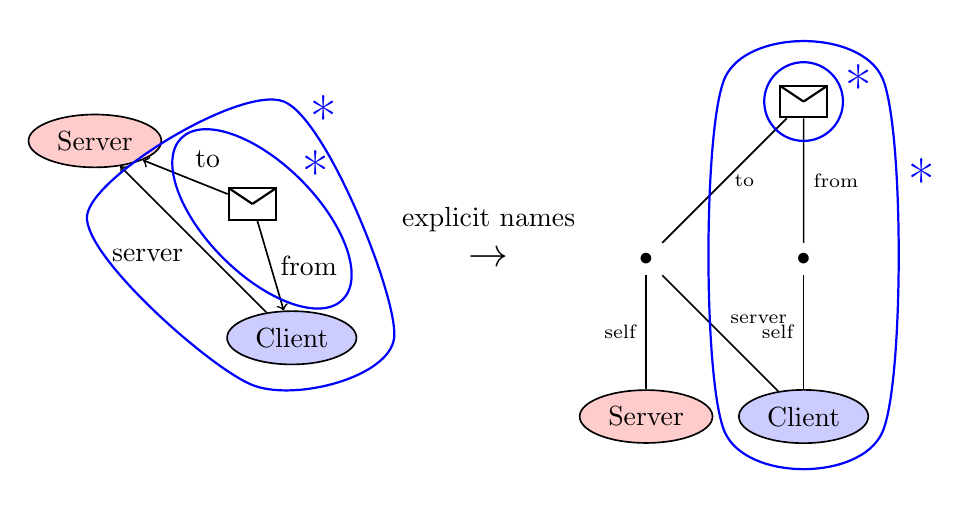
\begin{tikzpicture}[semithick]

  \begin{scope}[xshift=-4cm,->]
  \node [draw,ellipse,fill=red!20]  (x) at ( 0, 0) {Server};

  \node [draw,ellipse,fill=blue!20] (m) at ( 2.5, -2.5) {Client};
  \path  (m) edge node [below left] {server} (x);
  
  \tikzMessageNode{mm}{2.0,-0.8}
  \path  (mm) edge node [right] {from} (m);
  \path  (mm) edge node [above right] {to} (x);

  \draw[thick,rotate=45,color=blue] (0.8,-2.2) ellipse (0.7 and 1.45);
  \node[text=blue] (star) at ( 2.8, -0.4) {{\huge *}};

  \draw[color=blue,thick] plot[smooth cycle] coordinates{(-0.1,-0.95) (2.4,0.5) (3.8,-2.5) (2,-3.1)};
  \node[text=blue] (star) at ( 2.9, 0.3) {{\huge *}};
  \end{scope}
  
  \begin{scope}[xshift=1cm,yshift=-1.5cm]
  \node at ( 0, 0.5) {explicit names};
  \node at ( 0, 0) {\Large $\rightarrow$};
  \end{scope}

  \begin{scope}[xshift=3cm, yshift=-3.5cm, node distance=2cm]

  \node [draw,ellipse,fill=red!20]  (x) at ( 0, 0) {Server};
  \node (nx) [above of=x] {$\bullet$};
  \path  (x) edge node [left] {\scriptsize self} (nx);

  \node [draw,ellipse,fill=blue!20] (m) [right of=x] {Client};
  \node (nm) [above of=m] {$\bullet$};
  \path  (m) edge node [left] {\scriptsize self} (nm);
  \path  (m) edge node [above right] {\scriptsize server} (nx);
  
  \tikzMessageNode{mm}{2.0,4}
  \path  (mm) edge node [right] {\scriptsize from} (nm);
  \path  (mm) edge node [right] {\scriptsize to} (nx);

  \draw[thick,color=blue] (2,4) ellipse (0.5 and 0.5);
  \node[text=blue] (star) at ( 2.7, 4.2) {{\huge *}};

  \draw[color=blue,thick] plot[smooth cycle] coordinates{(1,4.3) (3,4.3) (3,-0.2) (1,-0.2)};
  \node[text=blue] (star) at ( 3.5, 3) {{\huge *}};
  \end{scope}

  \end{tikzpicture}
  \end{center}
  
\end{frame}

\begin{frame}
  \frametitle{Regular language of unranked trees for Client-Server (2)}
  \[(\nu x)(Server(x) \,|\, !(\nu y)(Client(y,x) | !Messages(x,y))) \]
  
  \begin{center}
  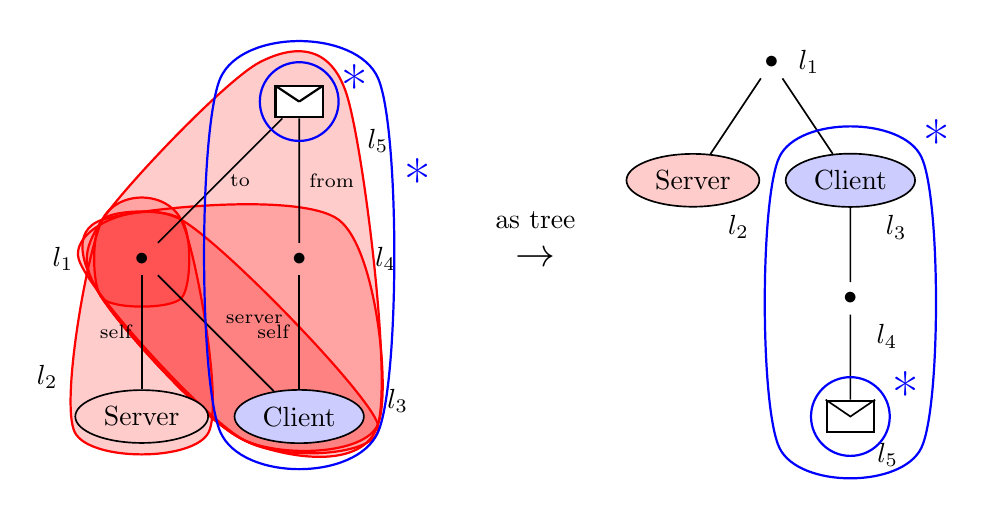
\begin{tikzpicture}[semithick]

  \begin{scope}[xshift=-5cm, yshift=-2cm, node distance=2cm]
  
  %labels
  %l_1
  \draw[color=red,fill=red,thick,fill opacity=0.2] plot[smooth cycle]
  coordinates{(-0.5,1.5) (-0.5,2.5) (0.5,2.5) (0.5,1.5)};
  \node at (-1,2) {$l_1$};
  %l_2
  \draw[color=red,fill=red,thick,fill opacity=0.2] plot[smooth cycle]
  coordinates{(-0.85,-0.2) (-0.5,2.5) (0.5,2.5) (0.85,-0.2)};
  \node at (-1.2,0.5) {$l_2$};
  %l_3
  \draw[color=red,fill=red,thick,fill opacity=0.2] plot[smooth cycle]
  coordinates{(1.3,-0.3) (-0.8,2) (0.5,2.5) (3,-0.1)};
  \node at (3.25,0.2) {$l_3$};
  %l_4
  \draw[color=red,fill=red,thick,fill opacity=0.2] plot[smooth cycle]
  coordinates{(-0.5,1.5) (-0.5,2.5) (2.5,2.5) (3,-0.1) (1.3,-0.3)};
  \node at (3.1,2) {$l_4$};
  %l_5
  \draw[color=red,fill=red,thick,fill opacity=0.2] plot[smooth cycle]
  coordinates{(-0.5,1.5) (-0.5,2.5) (1.5,4.5) (2.6,4.1) (3,-0.1) (1.3,-0.3)};
  \node at (3,3.5) {$l_5$};

  \node [draw,ellipse,fill=red!20]  (x) at ( 0, 0) {Server};
  \node (nx) [above of=x] {$\bullet$};
  \path  (x) edge node [left] {\scriptsize self} (nx);

  \node [draw,ellipse,fill=blue!20] (m) [right of=x] {Client};
  \node (nm) [above of=m] {$\bullet$};
  \path  (m) edge node [left] {\scriptsize self} (nm);
  \path  (m) edge node [above right] {\scriptsize server} (nx);
  
  \tikzMessageNode{mm}{2.0,4}
  \path  (mm) edge node [right] {\scriptsize from} (nm);
  \path  (mm) edge node [right] {\scriptsize to} (nx);

  \draw[thick,color=blue] (2,4) ellipse (0.5 and 0.5);
  \node[text=blue] (star) at ( 2.7, 4.2) {{\huge *}};

  \draw[color=blue,thick] plot[smooth cycle] coordinates{(1,4.3) (3,4.3) (3,-0.2) (1,-0.2)};
  \node[text=blue] (star) at ( 3.5, 3) {{\huge *}};
  \end{scope}

  \begin{scope}
  \node at ( 0, 0.5) {as tree};
  \node at ( 0, 0) {\Large $\rightarrow$};
  \end{scope}
  
  \begin{scope}[xshift=3cm, yshift=2.5cm,level 1/.style={sibling distance=2cm}, node distance=1.5cm]
  \node[label={right:$l_1$}] {$\bullet$}
    child{node[draw,ellipse,fill=red!20,label={below right:$l_2$}] {Server}}
    child{node[draw,ellipse,fill=blue!20,label={below right:$l_3$}] {Client}
      child{node[label={below right:$l_4$}] {$\bullet$}
        child{node[draw,thick,fill=white,rectangle,inner sep=0pt,minimum height=0.4cm,minimum width=0.6cm,label={below right:$l_5$}] (m) {} }}
    }
  ;
  \draw (m.north west) -- (m.center) -- (m.north east);
  
  \draw[thick,color=blue] (1,-4.5) ellipse (0.5 and 0.5);
  \node[text=blue] (star) at ( 1.7, -4.2) {{\huge *}};

  \draw[color=blue,thick] plot[smooth cycle] coordinates{(0.1,-1.2) (1.9,-1.2) (1.9,-4.9) (0.1,-4.9)};
  \node[text=blue] (star) at ( 2.1, -1) {{\huge *}};
  \end{scope}

  \end{tikzpicture}
  \end{center}
  
\end{frame}

\begin{frame}
  \frametitle{Regular language of unranked trees for Client-Server (3)}
  \[(\nu x)(Server(x) \,|\, !(\nu y)(Client(y,x) | !Messages(x,y))) \]
  
  \begin{center}
  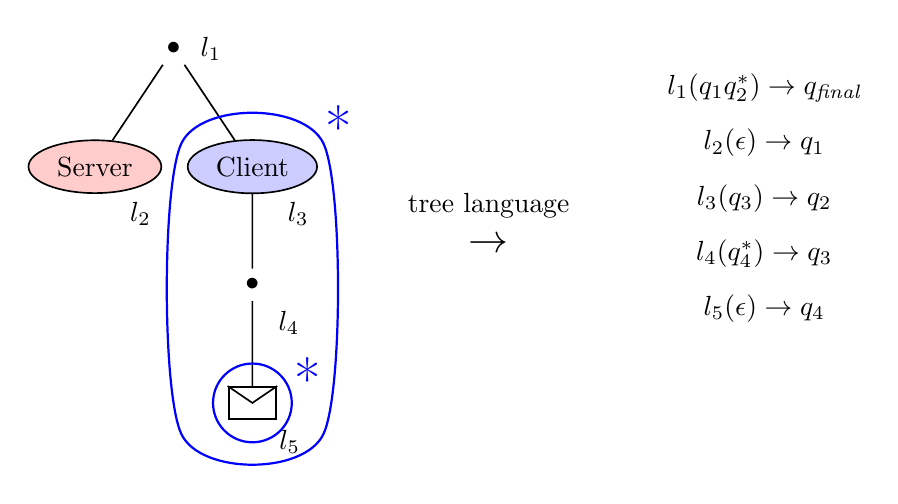
\begin{tikzpicture}[semithick]

  \begin{scope}[xshift=-4cm, yshift=2.5cm,level 1/.style={sibling distance=2cm}, node distance=1.5cm]
  \node[label={right:$l_1$}] {$\bullet$}
    child{node[draw,ellipse,fill=red!20,label={below right:$l_2$}] {Server}}
    child{node[draw,ellipse,fill=blue!20,label={below right:$l_3$}] {Client}
      child{node[label={below right:$l_4$}] {$\bullet$}
        child{node[draw,thick,fill=white,rectangle,inner sep=0pt,minimum height=0.4cm,minimum width=0.6cm,label={below right:$l_5$}] (m) {} }}
    }
  ;
  \draw (m.north west) -- (m.center) -- (m.north east);
  
  \draw[thick,color=blue] (1,-4.5) ellipse (0.5 and 0.5);
  \node[text=blue] (star) at ( 1.7, -4.2) {{\huge *}};

  \draw[color=blue,thick] plot[smooth cycle] coordinates{(0.1,-1.2) (1.9,-1.2) (1.9,-4.9) (0.1,-4.9)};
  \node[text=blue] (star) at ( 2.1, -1) {{\huge *}};
  \end{scope}

  \begin{scope}
  \node at ( 0, 0.5) {tree language};
  \node at ( 0, 0) {\Large $\rightarrow$};
  \end{scope}
  
  \begin{scope}[xshift=3.5cm, yshift=2cm,node distance=7mm]
  \node (r1)                {$l_1(q_1 q_2^*) \rightarrow q_{\textit{final}}$};
  \node (r2) [below of=r1]  {$l_2(\epsilon) \rightarrow q_1$};
  \node (r3) [below of=r2]  {$l_3(q_3) \rightarrow q_2$};
  \node (r4) [below of=r3]  {$l_4(q_4^*) \rightarrow q_3$};
  \node (r5) [below of=r4]  {$l_5(\epsilon) \rightarrow q_4$};
  \end{scope}
  \end{tikzpicture}
  \end{center}
  
\end{frame}

\begin{frame}[fragile]
  \frametitle{Further Work}
  %\begin{itemize}
  %\item \cite{Meyer08OnBoundednessInDepth} introduces depth-bounded systems.
  %\item \cite{DBLP:conf/concur/MeyerG09} precises the relation between \pical{} processes and finite p/t Petri nets in terms of computational expressiveness.
  %\item \cite{GeeraertsETAL06ExpandEnlargeCheck} gives a forward algorithm to decide the coverability problem of WSTS.
  %\item \cite{FinkelGoubaultLarrecq09ForwardAnalysisForWSTS} provides a theoretical framework for manipulating downward-closed sets.
  %\item
  We started an implemention to compute (an over-approximation of) the cover using \cite{DBLP:conf/icalp/FinkelG09}.% by mixing widening and acceleration.
  %\item \cite{DBLP:conf/vmcai/GantyRB06} represents downward-closed sets as complements of upward-closed sets.
  %\item Fragments of the \pical{} that are subsumed by depth-bounded processes:
  %  \cite{DBLP:journals/njc/AmadioM02,DBLP:conf/concur/Dam93} (defined syntactically),
  %  \cite{KOstrovsky05,DBLP:journals/tcs/Sangiorgi96a,DBLP:conf/icalp/BusiGZ03} (in terms of type systems).
  %\item \cite{BauerWilhelm07StaticAnalysisOfDCS} developed an shape analysis for graph rewriting systems with star-like shape.
  %\item $\ldots$
  %\end{itemize}

\begin{figure}
\begin{minipage}{0.55\linewidth} % A minipage that covers half the page
{\scriptsize
\begin{verbatim}
Equations:
----------------------------------------
client1(A, B) = (A().(client1(A, B) |
                    request1(B, A)))
answer1(A) = (A<>.0)
new1(A) = (A<>.0)
request1(A, B) = (A<B>.0)
server(A, B) = (A(C).(answer1(C) |
                      server(A, B)) +
                B().(ny D)
                      (client1(D, A) |
                       answer1(D) |
                       new1(B) |
                       server(A, B)))

Initial configuration:
----------------------------------------
(ny A, B)
    (new1(A) |
     server(B, A))
\end{verbatim}
}
\end{minipage}
\hspace{0.5cm} % To get a little bit of space between the figures
\begin{minipage}{0.35\linewidth}
{\scriptsize
\begin{verbatim}
Computed cover:

(ny A, B)
    (!((ny C)
         (answer1(C) |
         client1(C, B))) |
    !((ny D)
         (client1(D, B) |
         request1(B, D))) |
    new1(A) |
    server(B, A))
\end{verbatim}
}
\end{minipage}
\end{figure}

\end{frame} 


\begin{frame} 
  \frametitle{Recap}
  \begin{center}
    Coverability is decidable for depth-bounded processes.
  \end{center}
  \begin{itemize}
  \item We provide an ADL for depth-bounded processes;
  \item prepared the ground for a spectrum of forward algorithms for depth-bounded processes.
  \end{itemize}
\end{frame} 

\begin{frame} 
  \frametitle{}
  \begin{center}
  {\Large Questions ?}
  \end{center}
\end{frame} 

\begin{frame}
  \frametitle{Depth-bounded systems \cite{Meyer08OnBoundednessInDepth}}
  Nesting of names:
  \begin{eqnarray*}
  & & \nest((\nu x)P) = 1 + \nest(P),\\
  & & \nest(P_1 \mid P_2) = \max\set{\nest(P_1),\nest(P_2)},\\
  & & \ldots
  \end{eqnarray*}

  The Depth of a configuration:
  \[\depth(P) = \min\pset{\nest(Q)}{Q \equiv P}\]

  A process $\process$ is \emph{depth-bounded} if:
  \[\exists k \in \mathbb{N}, ~ \forall P \in \Reach(\process), ~ \depth(P) \leq k\]

  (Concretely: it is not possible to make an infinite memory.)
\end{frame}

\begin{frame}
  \frametitle{Backward analysis: aliasing problem}
  Backward analysis has to guess the exchanged names of each reduction step.\\
  $\rightarrow$ explosion in the nondeterminism.

  \begin{center}
  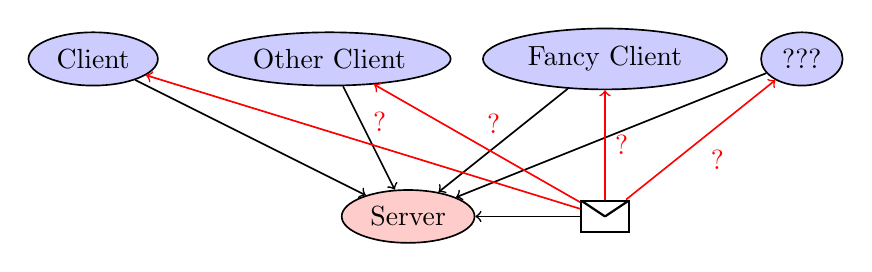
\begin{tikzpicture}[semithick, ->, node distance=2cm]
  \node [draw,ellipse,fill=red!20]  (x) at ( -1, 0) {Server};

  %replication of clients
  \node [draw,ellipse,fill=blue!20] (ni) at (-5, 2) {Client};
  \path  (ni) edge node [left] {} (x);
  \node [draw,ellipse,fill=blue!20] (n1) at (-2, 2) {Other Client};
  \path  (n1) edge (x);
  \node [draw,ellipse,fill=blue!20] (n2) at (1.5, 2) {Fancy Client};
  \path  (n2) edge (x);
  \node [draw,ellipse,fill=blue!20] (n3) at (4, 2) {???};
  \path  (n3) edge (x);
  
  \tikzMessageNode{mm}{1.5,0}
  \path  (mm) edge node [above right] {} (x);
  \path[red]  (mm) edge node [above right] {?} (ni);
  \path[red]  (mm) edge node [above right] {?} (n1);
  \path[red]  (mm) edge node [right] {?} (n2);
  \path[red]  (mm) edge node [below right] {?} (n3);

  \end{tikzpicture}
  \end{center}
\end{frame}

\begin{frame}
  \frametitle{Closure of a tree}

  \begin{center}
  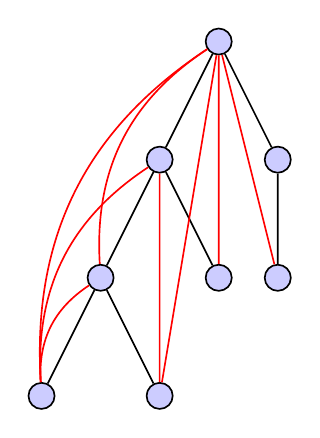
\begin{tikzpicture}[semithick]
    \node[circle,draw,fill=blue!20] (n1) {}
      child {node[circle,draw,fill=blue!20] (n2) {}
        child {node[circle,draw,fill=blue!20] (n4) {}
          child {node[circle,draw,fill=blue!20] (n8) {} }
          child {node[circle,draw,fill=blue!20] (n9) {} }
        }
        child {node[circle,draw,fill=blue!20] (n5) {}
        }
      }
      child {node[circle,draw,fill=blue!20] (n3) {}
        child {node[circle,draw,fill=blue!20] (n7) {}
        }
      };
    \path[red]
      (n1) edge [bend right] (n4)
      (n1) edge [bend right] (n8)
      (n2) edge [bend right] (n8)
      (n4) edge [bend right] (n8)
      (n2) edge (n9)
      (n1) edge (n9)
      (n1) edge (n5)
      (n1) edge (n7)
    ;
  \end{tikzpicture}
  \end{center}
  Add \alert{edges} according to the transitive closure of the parent relation.

  \vspace{10pt}

  Every (undirected) graph is included in the closure of some tree.

\end{frame}

\begin{frame}[allowframebreaks]{References}
  \frametitle{}
  {\tiny
  %\bibliographystyle{annotate}
  %\bibliographystyle{plainnat}
  \bibliographystyle{cell}
  %\bibliographystyle{abbrvnat}
  \bibliography{biblio}
  }
\end{frame}

\end{document}
